\documentclass[10pt]{article}
\usepackage[utf8]{inputenc}
\usepackage[a4paper,left=3cm,right=3cm,top=3cm,bottom=3cm]{geometry}
\usepackage[german]{babel}
\usepackage{amsmath}
\usepackage{amssymb}
\usepackage{bm}
\usepackage[hidelinks]{hyperref}
\usepackage{graphicx}
\usepackage[font=small,labelfont=bf]{caption}
\usepackage[toc]{glossaries}  % needs to be after hyperref

% Adjust paragraph and text spacings
\setlength\parindent{0pt}
\setlength{\parskip}{8pt}
\renewcommand{\arraystretch}{1.5}
\renewcommand{\baselinestretch}{1.5}

% Describe title
\title{Evocracy Whitepaper}
\author{Carlo Michaelis, Patrick Charrier, Jannik Luboeinski}
\date{2020-01-28\\ (v1.0)}

% Glossary entries
\newglossaryentry{thema}{
  name=Thema, plural=Themen,
  description={Eine bestimmte abgegrenzte Problemstellung, über die eine Diskussion stattfinden soll}
}
\newglossaryentry{benutzer}{
  name=Benutzer, plural=Benutzer,
  description={Eine Person, die sich in einer OpenEvocracy-Installation registriert hat},
}
\newglossaryentry{teilnehmer}{
  name=Teilnehmer, plural=Teilnehmer,
  description={Ein Benutzer, der für ein Thema einen validen Vorschlag eingereicht hat (das Gegenteil ist der Beobachter)},
}
\newglossaryentry{zielgruppe}{
  name=Zielgruppe, plural=Zielgruppen,
  description={Eine Gruppe von Benutzern, die berechtigt sind zu einem bestimmten Thema einen Vorschlag schreiben zu düfen},
}
\newglossaryentry{bezugsgruppe}{
  name=Bezugsgruppe, plural=Bezugsgruppen,
  description={Dezentral organisierte Gruppe, die einem bestimmten Zweck dient},
}
\newglossaryentry{interessengruppe}{
  name=Interessengruppe, plural=Interessengruppen,
  description={Zentral organisierte Gruppe, die einem bestimmten Zweck dient},
}
\newglossaryentry{pot-teilnehmer}{
  name=potenzieller Teilnehmer, plural=potenzielle Teilnehmer,
  description={Ein Benutzer, der für ein bestimmtes Thema berechtigt ist einen Vorschlag einreichen zu können},
}
\newglossaryentry{relevanz}{ % Substantiv + Adjektiv ("relevant")
  name=Relevanz, plural=Relevanzen,
  description={Wert, den die Benutzer einenm Thema zuweisen können und der dazu führt, dass die Diskussion zu einem Thema gestartet wird, wenn er oberhalb der Relevanzschwelle liegt},
}
\newglossaryentry{relevanzmarkierung}{ % Substantiv + Adverb ("als relevant markieren")
  name=Relevanzmarkierung, plural=Relevanzmarkierungen,
  description={Die Relevanzmarkierung eines Benutzers für ein Thema erhöht den Wert der Relevanz um 1},
}
\newglossaryentry{vorschlag}{
  name=Vorschlag, plural=Vorschläge,
  description={Individueller Lösungsansatz eines Benutzers für ein bestimmtes Thema},
}
\newglossaryentry{vorschlagphase}{
  name=Vorschlagphase,
  description={Phase eines Themas, in der Vorschläge eingereicht werden können},
}
\newglossaryentry{konsensphase}{
  name=Konsensphase,
  description={Phase eines Themas, in die Teilnehmer eines Themas in Gruppen Lösungen erarbeiten; besteht aus verschiedenen aufeinanderfolgenden Stufen},
}
\newglossaryentry{beobachter}{
  name=Beobachter, plural=Beobachter,
  description={Benutzer, der bei einem Thema keinen Vorschlag eingereicht hat (das Gegenteil ist der Teilnehmer)},
}
\newglossaryentry{gruppe}{
  name=Gruppe, plural=Gruppen,
  description={Die Teilnehmer werden in den verschiedenen Stufen der Konsensphase in Gruppen aufgeteilt},
}
\newglossaryentry{stufe}{
  name=Stufe, plural=Stufen,
  description={Unterphase der Konsensphase, deren Anzahl sich durch die Anzahl der Teilnehmer und die Größe der Gruppen ergibt},
}
\newglossaryentry{mitglied}{
  name=Mitglied, plural=Mitglieder,
  description={Bezeichnet die Teilnehmer einer Gruppe},
}
\newglossaryentry{koll-dok}{
  name=kollaboratives Dokument, plural=kollaborative Dokumente,
  description={Dokument, das von den Mitgliedern einer Gruppe gemeinsam bearbeitet wird},
}
\newglossaryentry{delegierter}{
  name=Delegierter, plural=Delegierte,
  description={Für die nächste Stufe gewählter Vertreter einer Gruppe},
}
\newglossaryentry{konsensgrad}{
  name=Konsensgrad,
  description={Wert, der angibt, wie viel Zustimmung das abschließende Dokument bei allen Teilnehmern des Themas besitzt},
}
\newglossaryentry{standort}{
  name=Standort, plural=Standorte,
  description={Wohnort oder Aufenthaltsort eines Benutzers, der von anderen Benutzern bestätigt werden kann und ab einer bestimmten Anzahl von Bestätigungen verifiziert ist; verifizierte Standorte ermöglichen einen Zugang zu Bezugsgruppen und Themen},
}
\newglossaryentry{laufzeitparameter}{
  name=Laufzeitparameter, plural=Laufzeitparameter,
  description={Parameter, die zur Laufzeit des Systems durch Benutzer demokratisch und dezentral ausgewählt werden und das System selbt verändern},
}
\newglossaryentry{autor}{
  name=Autor, plural=Autoren,
  description={Benutzer, der ein bestimmtes Thema erstellt hat},
}
\newglossaryentry{post}{
  name=Post, plural=Posts,
  description={Beitrag eines Benutzers, der an eine Bezugsgruppe, eine Interessengruppe und/oder Follower gerichtet ist},
}
\newglossaryentry{follower}{
  name=Follower, plural=Follower,
  description={Benutzer, der an den Posts eines anderen Benutzers interessiert ist und diesem anonym ``folgt''},
}
\newglossaryentry{empf-gruppe}{
  name=Empfängergruppe, plural=Empfängergruppen,
  description={Eine Gruppe von Benutzern, die Zugang zu einem bestimmten Post im sozialen Netzwerk erhalten},
}
\newglossaryentry{genosse}{
  name=Genosse, plural=Genossen,
  description={Benutzer, der Teil einer bestimmten Interessengruppe ist},
}


% Format glossary entries to italic
\renewcommand{\glstextformat}[1]{\textit{#1}}

% Generate glossary
\makeglossaries

\begin{document}

%\maketitle

\begin{center}

\vspace*{1.5cm}
{\Huge Evocracy Whitepaper}
\vspace*{1.5cm}

{\large Carlo Michaelis, Patrick Charrier, Jannik Luboeinski}

develop@openevocracy.org\\
\href{https://openevocracy.org/}{https://openevocracy.org}
\vspace*{1cm}

{\large 2020-01-28}

(v1.0)
\end{center}

\vspace*{\fill}

\begin{center}
Das Whitepaper ist unter folgender Lizenz veröffentlicht:\\ \href{https://creativecommons.org/licenses/by/4.0/}{Attribution 4.0 International (CC BY 4.0)}
\end{center}

\thispagestyle{empty}
\newpage

%%%%%%%%%%%%%%%%%%%%
%%%%% ABSTRACT %%%%%
%%%%%%%%%%%%%%%%%%%%

\section*{Abstract}

Evocracy ist ein Konzept zur Organisation demokratischer Entscheidungsfindung, welches zu diesem Zweck moderne Informationstechnologie verwendet. Ziel ist, eine hohe Qualität von Entscheidungen zu ermöglichen, Entscheidungsprozesse zu dezentralisieren, sowie gleichzeitig möglichst viel Anonymität und Sicherheit zu gewährleisten. Im Zentrum des Konzeptes stehen von Benutzern erstellte Themen. Diese definieren eine Frage- oder Problemstellung, über die eine Entscheidung getroffen werden soll.

Diskussionen zu einem Thema werden in kleine Gruppen ausgelagert, deren Mitglieder jeweils an einem Dokument arbeiten. Aufgrund der kleinen Gruppen hat jede Idee die Chance, berücksichtigt zu werden. Basierend auf ihrem themenspezifischen Wissen und ihrer Fähigkeit, Ideen zu vereinen, werden Delegierte der Gruppen in höhere Stufen gewählt, wo sie mit anderen gewählten Delegierten erneut kleine Gruppen bilden. Die Anzahl der Teilnehmer und Gruppen reduziert sich damit von Stufe zu Stufe, bis ein einziges Dokument übrig bleibt. Durch den Prozess werden diejenigen Ideen stärker berücksichtigt, die sich über mehrere Gruppen hinweg in den Diskussionen als vernünftig und konsensfähig erweisen. Durch diesen selbstorganisierenden Prozess werden gute Ideen in einem evolutionären Sinn selektiert.

Evocracy ist frei von expliziten Autoritäten, alle Benutzer besitzen die gleichen Rechte. Jeder Benutzer hat das Recht Themen vorzuschlagen und potenziell an jedem Thema teilzunehmen. Um Missbrauch zu verhindern, werden Standort und Authentizität eines Benutzers dezentral, d.h. durch gegenseitige Bestätigung und Bewertung, verifiziert. Es gibt jedoch keine Möglichkeit, Benutzer zu identifizieren. Jedes Thema ist einer von vielen möglichen Zielgruppen zugeordnet, welche sich unabhängig von bestehenden Strukturen (wie Staaten, Gemeinden usw.) dynamisch aus den Beziehungen der Standorte der Benutzer ergeben können.
\newpage

\tableofcontents
\newpage

%%%%%%%%%%%%%%%%%%%%%%
%%%%% EINLEITUNG %%%%%
%%%%%%%%%%%%%%%%%%%%%%

\section{Einleitung}

Das Evocracy-Konzept befasst sich ausschließlich mit der Entscheidungsfindung, ist also vergleichbar mit der Legislative. Dabei sind zwei grundsätzliche Probleme zu lösen:

\begin{enumerate}
    \item Wie können wir herausfinden, ob ein \gls{thema} \glsdisp{relevanz}{relevant} ist?
    \item Wie können wir zu einem \gls{thema} eine gute Entscheidung finden? 
\end{enumerate}

Der Ansatz von Evocracy ist, dass \glspl{benutzer} für sie \glsdisp{relevanz}{relevante} \glspl{thema} markieren können, und dass im Laufe des Entscheidungsprozesses zu einem bestimmten \gls{thema} genau diejenigen \glspl{teilnehmer} an Einfluss gewinnen, die inhaltlich viel beitragen können und bezüglich des \glsdisp{thema}{Themas} eine hohe Sensibilität aufweisen. Vom evolutionären Charakter dieser Idee und der basisdemokratischen Beteiligung aller \glspl{teilnehmer} leitet sich der Name Evocracy ab. Die zugehörige Open-Source-Software nennen wir OpenEvocracy.

Aus Gründen der besseren Lesbarkeit wird auf die Verwendung mehrerer geschlechtsspezifischer Sprachformen verzichtet. Sämtliche Personenbezeichnungen gelten gleichermaßen für alle Geschlechter.

%%%%%%%%%%%%%%%%%%%
%%%%% PROZESS %%%%%
%%%%%%%%%%%%%%%%%%%

\section{Entscheidungsfindungsprozess}

Zur Findung einer Entscheidung durchläuft ein \gls{thema} verschiedene Phasen, die im Folgenden erläutert werden.

\subsection{Aufstellen und Selektieren von Themen (Auswahlphase)}

\begin{figure}[!t]
	\centering
	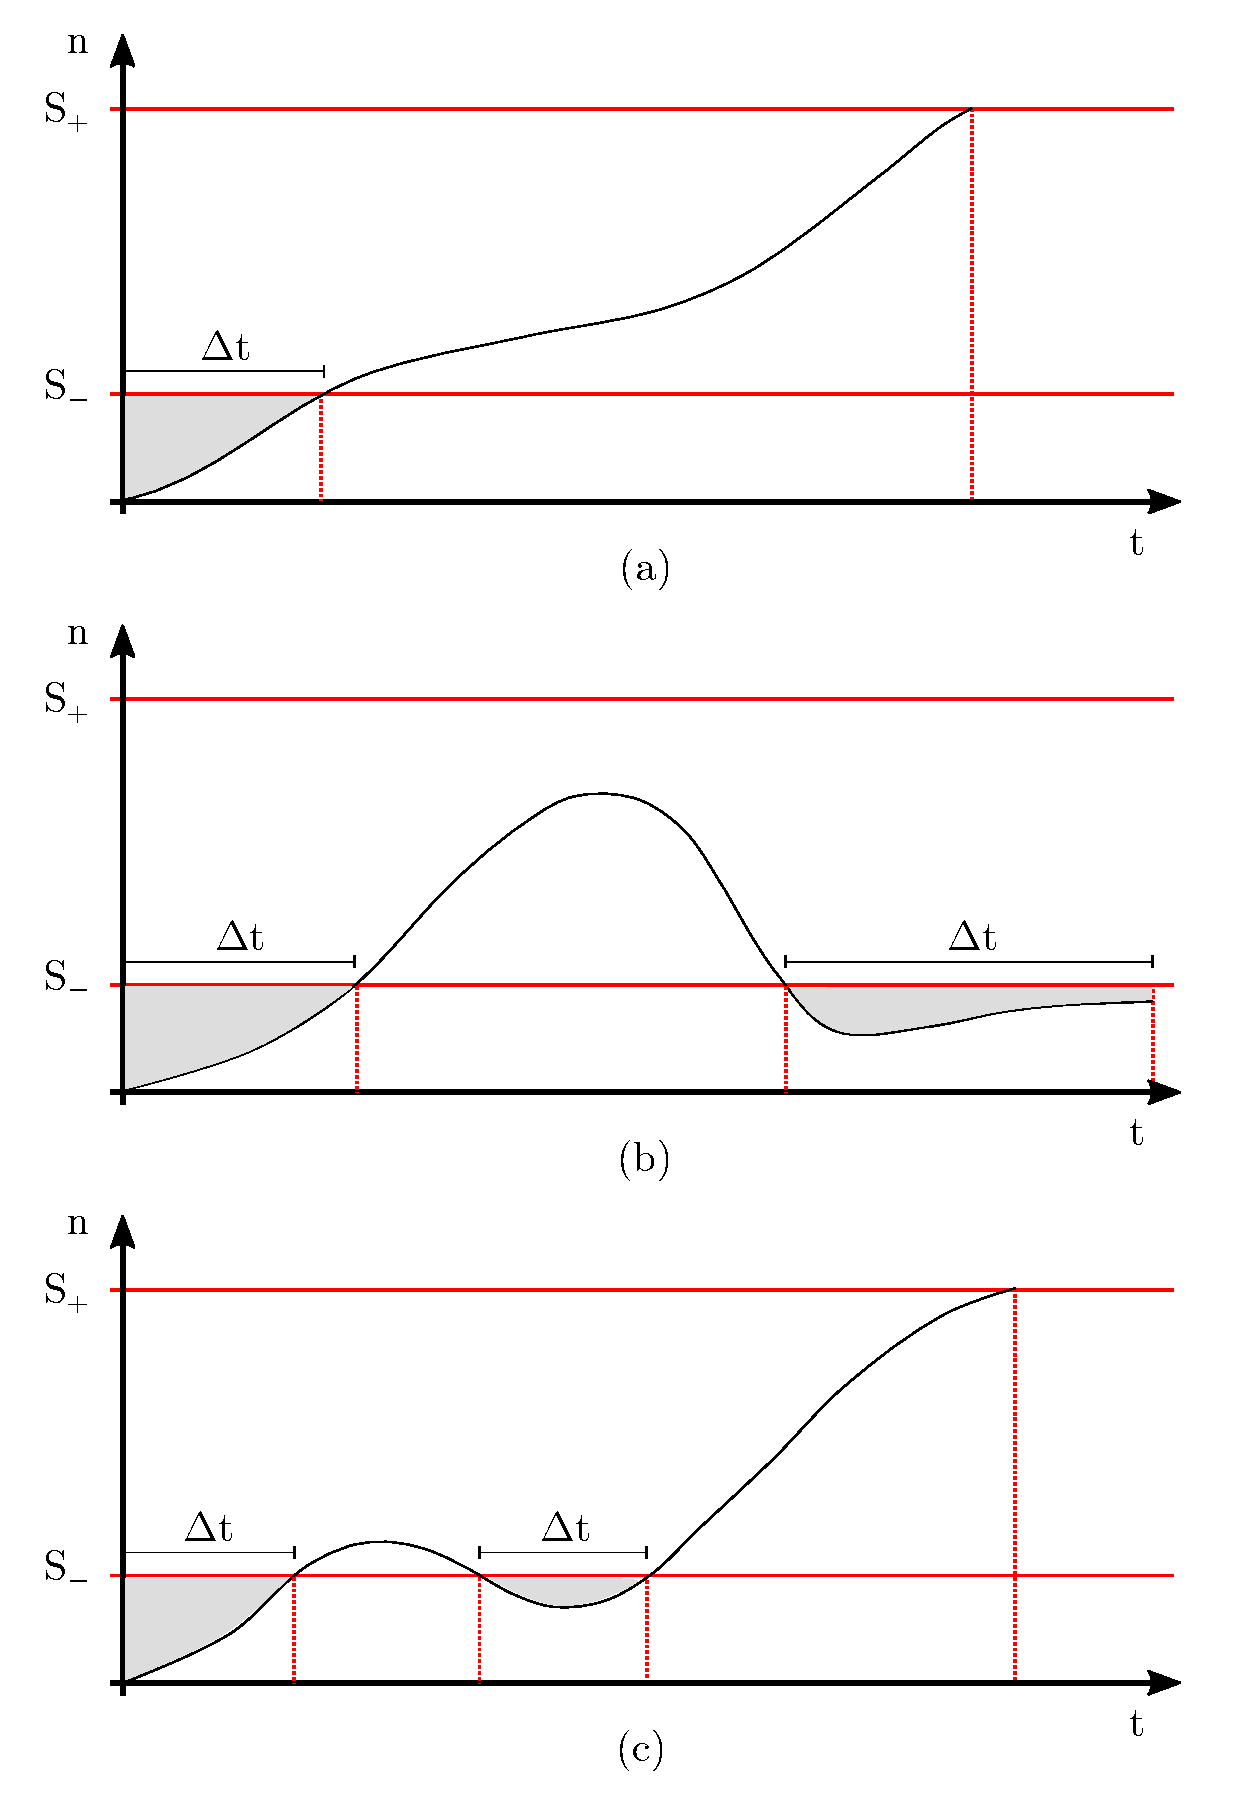
\includegraphics[width=0.5\textwidth]{schwellen_v3.pdf}
	\caption{Die Schwellenwerte für die Anzahl der notwendigen Relevanzmarkierungen bestimmen, wann ein Thema zur Diskussion angenommen wird. Es können viele verschiedene Verläufe der Relevanzmarkierungen auftreten, drei Beispiele sind hier gezeigt: (a) Die Anzahl der Relevanzmarkierungen nimmt stetig zu und überschreitet schließlich den oberen Schwellenwert, sodass das Thema angenommen wird. (b) Die Anzahl der Relevanzmarkierungen nimmt zunächst zu, fällt dann aber wieder ab. Nachdem sie für die Zeit $\Delta t \geq \Delta t_\text{reject}$ unter dem unteren Schwellenwert gelegen hat, wird das Thema verworfen. (c) Die Anzahl der Relevanzmarkierungen nimmt zunächst zu, fällt dann vorübergehend wieder ab, liegt für eine Zeit $\Delta t < \Delta t_\text{reject}$ unterhalb des unteren Schwellenwertes, und nimmt dann aber wieder zu bis sie den oberen Schwellenwert überschreitet. Das Thema wird angenommen.} \label{fig.schwellenwerte}
\end{figure}

Grundsätzlich hat jeder \gls{benutzer} die Möglichkeit, ein \gls{thema} aufzustellen. Ein \gls{thema} wird durch eine Überschrift, einen Beschreibungstext und eine \gls{zielgruppe} (entweder eine \gls{bezugsgruppe} oder \gls{interessengruppe} wie ``Kassel'', ``Hessen'', ``Rockfestival 2018'' oder ``Personalabteilung'', oder ein bestimmter geografischer Bereich; siehe Abb. \ref{fig.zielgruppen_empfaengergruppen}) definiert. Die Art der \glspl{bezugsgruppe} und/oder \glspl{interessengruppe} hängt vom jeweiligen Einsatzbereich der OpenEvocracy-Installation ab. Alle \glspl{benutzer}, die der \gls{zielgruppe} angehören, können am \gls{thema} teilnehmen, sie sind also \glspl{pot-teilnehmer}.

Alle \glspl{benutzer} können zu jedem \gls{thema} Meinungen und Kommentare beitragen. Um die \glspl{thema} möglichst frei von persönlichen Präferenzen zu halten, kann ihnen Literatur, z.B. wissenschaftliche Studien, zugeordnet werden. So wird gemeinsam dazu beigetragen, dass Interessenten einen möglichst differenzierten und klaren Eindruck eines spezifischen \glsdisp{thema}{Themas} bekommen.

Um eine Themenauswahl zu treffen, haben alle \glspl{benutzer} die Möglichkeit, die \gls{relevanz} der aufgestellten \glspl{thema} zu beurteilen. Zu diesem Zweck werden zwei Schwellenwerte definiert. Diese sind abhängig von der Bezugsgröße $N_{\text{ref}} \le N_{\text{tot}}$, wobei $N_{\text{tot}}$ die Anzahl aller \glspl{benutzer} und $N_{\text{ref}}$ die Anzahl der \glsdisp{pot-teilnehmer}{potenziellen Teilnehmer} ist. Die Anzahl der \glspl{relevanzmarkierung} wird mit $K$ bezeichnet. Die \gls{relevanzmarkierung} eines \glsdisp{benutzer}{Benutzers} verfällt, wenn dieser für einen bestimmten Zeitraum (z. B. 6 Monate) das \gls{thema} nicht mehr aufgerufen hat und seine \gls{relevanzmarkierung} nicht erneuert. Erreicht das Verhältnis $K/N_{\text{ref}}$ für ein \gls{thema} einen bestimmten oberen Schwellenwert, so wird dieses \gls{thema} als \glsdisp{relevanz}{relevant} betrachtet und zur Diskussion freigegeben. \glsdisp{relevanz}{Irrelevante} \glspl{thema}, für die $K/N_{\text{ref}}$ einen unteren Schwellenwert unterschreitet, werden an dieser Stelle aussortiert. Dieser Prozess wird als Auswahlphase bezeichnet, Beispiele sind in Abb. \ref{fig.schwellenwerte} gezeigt.

Die Schwellenwerte sind wie folgt definiert:

\begin{itemize}
    \item \textbf{Oberer Schwellenwert}: Ist $K/N_\text{ref} \geq S_+$, wobei $S_+$ der obere Schwellenwert ist, so wird das \gls{thema} angenommen.
    \item \textbf{Unterer Schwellenwert}: Bleibt $K/N_\text{ref}$ für einen Zeitraum $\Delta t \geq \Delta t_\text{reject}$ unter dem Schwellenwert $S_-$, so wird das \gls{thema} verworfen. Wird $S_-$ erneut innerhalb von $\Delta t < \Delta t_\text{reject}$ überschritten, so wird $\Delta t$ zurückgesetzt, d.h. $\Delta t=0$.
\end{itemize}

\subsection{Vorschläge (Vorschlagphase)}

Wenn ein \gls{thema} zur Diskussion angenommen wurde, hat jeder \gls{benutzer} die Möglichkeit, einen eigenen \gls{vorschlag} zu dem \gls{thema} zu verfassen. Neben konkreten Lösungsvorschlägen können auch schlicht Meinungen, Wünsche oder Befürchtung eingebracht werden. Die Bearbeitung des eigenen \glsdisp{vorschlag}{Vorschlags} ist auf den Zeitraum $T_P$ beschränkt.

Eine Mindestwortanzahl $N_P$ des \glsdisp{vorschlag}{Vorschlags} soll dazu motivieren, sich eigene Gedanken zum \gls{thema} zu machen und sich mit der gesammelten Literatur aus der Auswahlphase zu befassen. Um andererseits möglichst vielen \glsdisp{benutzer}{Benutzern} eine Teilnahme zu ermöglichen, soll die Mindestwortanzahl gering gehalten werden.

Wenn der Bearbeitungszeitraum $T_P$ abgelaufen ist, wird die \gls{vorschlagphase} beendet; weiteres Bearbeiten des eigenen \glsdisp{vorschlag}{Vorschlags} ist nicht mehr möglich. Alle Vorschläge mit mehr als $N_P$ Wörtern werden als gültig akzeptiert. \glspl{benutzer} mit gültigen Vorschlägen werden \glspl{teilnehmer} des Entscheidungsprozesses zu diesem \gls{thema}. Sie werden informiert und können an der folgenden \gls{konsensphase} teilnehmen. Alle anderen \glspl{benutzer}, die die Mindestwortanzahl $N_P$ nicht erreicht haben oder gar nicht erst einen \gls{vorschlag} angelegt haben, sind \glspl{beobachter} des Entscheidungsprozesses. \glspl{beobachter} können auf die folgende \gls{konsensphase} nur indirekt Einfluss nehmen, z.B. in Form von externen Foren (siehe unten).

\subsection{Entscheidungsfindung (Konsensphase)}

\begin{figure}[!t]
	\centering
	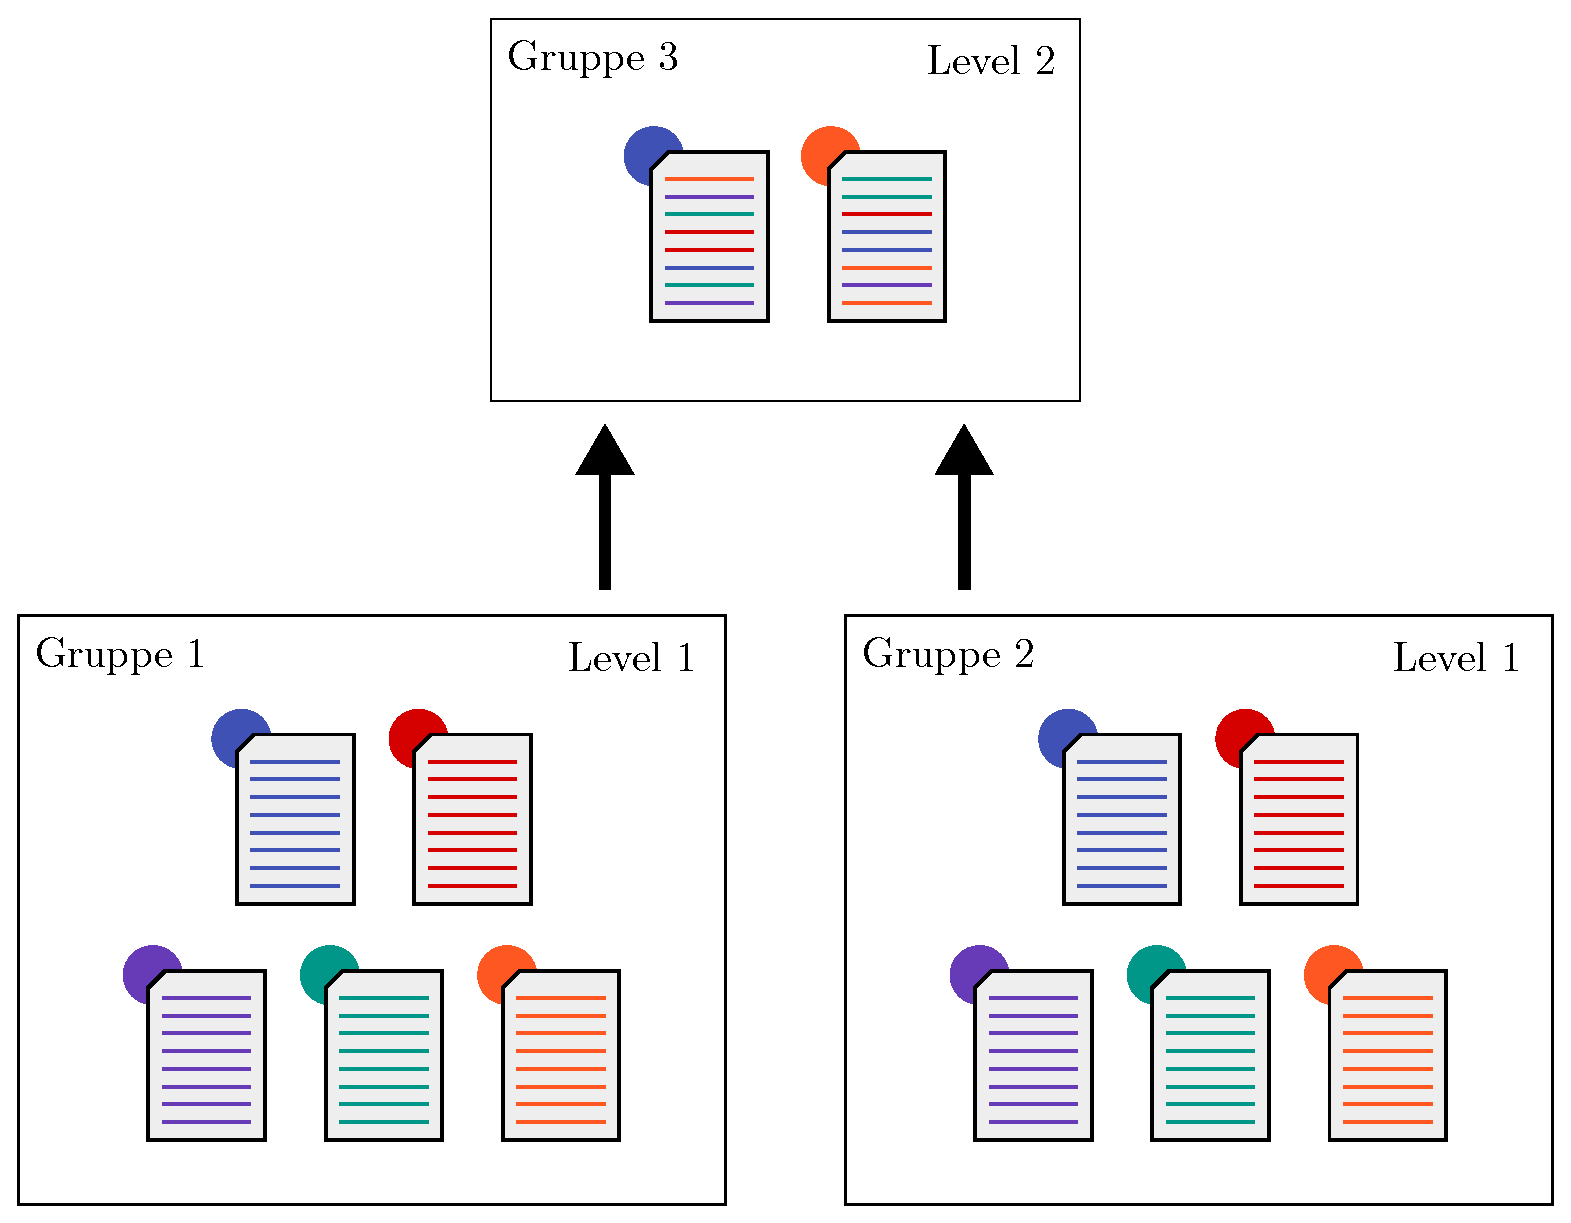
\includegraphics[width=0.8\textwidth]{evolution-tree_v2.pdf}
	\caption{Der evolutionäre Aufbau des Evocracy-Konzeptes. Die farbigen Punkte symbolisieren Mitglieder der Gruppe, die farbigen Zeilen in den Dokumenten symbolisieren deren Vorschläge. Innerhalb der Gruppen wird ein gemeinsamer Vorschlag erarbeitet, der von einem gewählten Delegierten in der nächsten Gruppe weiter bearbeitet wird. Gute Ideen aus früheren Gruppen bleiben in Gruppen späterer Level erhalten. Ebenso setzen sich Benutzer mit hohen Fähigkeiten durch.}
	\label{fig.evolution_tree}
\end{figure}

Alle \glspl{teilnehmer} werden in der ersten \gls{stufe} der \gls{konsensphase} per Zufall in \glspl{gruppe} der Größe $n_G$ (z.B. 5) eingeteilt. Kleine \glspl{gruppe} sind notwendig, da gemeinsame Diskussionen in großen \glspl{gruppe} von u.U. mehreren tausend \glsdisp{mitglied}{Mitgliedern} kaum möglich sind.

Innerhalb der \glspl{gruppe} werden per Zufall Namen und Farben vergeben. Diese gelten ausschließlich für diese \gls{gruppe} und sind nicht geschlechtsspezifisch. Die \glspl{mitglied} der \gls{gruppe} haben also jederzeit die Möglichkeit anonym zu bleiben. Sie können jedoch die Vorschläge aller anderen \glspl{mitglied} einsehen. Zudem wird ein leeres \gls{koll-dok} zur Verfügung gestellt, auf welches alle \glspl{mitglied} Schreibzugriff haben. Über Kommunikationsmittel (z.B. Chat, Forum, Terminfindung, Umfragen, Abstimmungen) können die \glspl{mitglied} über ihre Positionen diskutieren und Ergebnisse im \glsdisp{koll-dok}{kollaborativen Dokument} festhalten. Im Idealfall gelangt die \gls{gruppe} zu einem Konsens für die Lösung des Problems. Ist dies nicht der Fall, so steht es der \gls{gruppe} frei, auch Uneinigkeiten im Dokument festzuhalten.

Das \glsdisp{koll-dok}{kollaborative Dokument} soll in späteren Versionen von OpenEvocracy durch einen Machine-Learning-Algorithmus bereits initial mit einer Zusammenfassung der Inhalte aller \glspl{mitglied} gefüllt werden, so dass die \glspl{mitglied} bereits eine automatisch generierte Textvorlage haben. Der Algorithmus soll mit steigender Anzahl an \glspl{thema} optimiert werden.

Begleitend zur Formulierung des gemeinsamen \glsdisp{vorschlag}{Vorschlags} findet ein Bewertungsprozess statt. Die \glspl{mitglied} der \gls{gruppe} bewerten sich gegenseitig und sich selbst nach drei Kriterien.

\begin{itemize}
    \item \textbf{Kooperationsfähigkeit}: Wie gut kann das \gls{mitglied} kooperieren? Ist die Person fähig, Kompromisse einzugehen? Ist sie interessiert daran, alle Positionen zu hören und keine kategorisch auszuschließen? Hat die Person die Fähigkeit, für unterschiedliche Positionen eine neue Perspektive zu finden, die höhere Akzeptanz erfährt?
    \item \textbf{Wissen im Bereich des Themas}: Kann das \gls{mitglied} inhaltlich gut argumentieren? Ist die Person auf das \gls{thema} gut vorbereitet? Kann sich die Person differenziert und sachlich mit der Thematik auseinandersetzen?
    \item \textbf{Investierte Zeit}: Ist das \gls{mitglied} regelmäßig online? Beteiligt sich das \gls{mitglied} kontinuierlich am Diskussions- und Schreibprozess? Reagiert das \gls{mitglied} zeitnah auf Diskussionen im Chat und Forum?
\end{itemize}

Die \glsdisp{koll-dok}{kollaborativen Dokumente} der \glspl{gruppe} in einer \gls{stufe} der \gls{konsensphase} können nur für eine beschränkte Zeit bearbeitet werden. Nach Ablauf der Zeit wird der Bewertungsprozess automatisch ausgewertet, wobei ein \gls{delegierter} bestimmt wird, um die \gls{gruppe} zu vertreten. Alle anderen \glspl{mitglied} werden \glspl{beobachter} und haben keine direkte Einflussmöglichkeit mehr.

Die gewählten \glsdisp{delegierter}{Delegierten} werden erneut per Zufall \glspl{gruppe} der Größe $n_G$ zugewiesen, erhalten erneut ein \gls{koll-dok} und bekommen neue zufällig generierte Namen und Farben. Die \gls{konsensphase} erreicht damit eine neue \gls{stufe}. Der Prozess wird so lange durchgeführt, bis zuletzt eine einzelne \gls{gruppe} entsteht, die dann in der letzten \gls{stufe} das abschließende Dokument zum \gls{thema} erarbeitet.

\subsubsection{Externe Foren}

\glspl{beobachter} haben keinen Schreibzugriff auf die \glsdisp{koll-dok}{kollaborativen Dokumente} innerhalb der \glspl{gruppe}. Sie können diese Dokumente jedoch jederzeit einsehen. Neben dem \glsdisp{koll-dok}{kollaborativen Dokument} besitzt jede \gls{gruppe} ein Forum, in dem alle \glspl{benutzer} mitwirken können. Innerhalb eines Forums kann auf konkrete Textstellen im \glsdisp{koll-dok}{kollaborativen Dokument} der \gls{gruppe} Bezug genommen werden.

Die \glspl{mitglied} der jeweiligen \gls{gruppe} haben durch das Forum jederzeit die Möglichkeit, von externen Vorschlägen inspiriert zu werden und auf diese einzugehen, ohne dass die Diskussion innerhalb der \gls{gruppe} gestört wird. 

Einige Vorteile der Einbindung aller \glspl{benutzer} durch Foren sind:

\begin{itemize}
    \item Alle \glspl{benutzer}, insbesondere auch solche, die zu Beginn keinen \gls{vorschlag} eingereicht haben, können Ideen, Wünsche oder Kritik einbringen. Ideen, die im Laufe des Prozesses untergegangen sind, können noch einmal angebracht werden.
    \item Ein Transfer von Ideen zwischen unterschiedlichen \glspl{gruppe} wird ermöglicht, indem \glspl{benutzer} gute Ideen aus einer \gls{gruppe} im Forum einer anderen \gls{gruppe} einbringen können. Entscheidungen werden damit nicht nur vertikal zwischen den \glspl{stufe}, sondern auch horizontal zwischen den \glspl{gruppe} innerhalb einer \gls{stufe} optimiert.
    \item \glspl{teilnehmer} aus früheren \glspl{stufe} können die \glspl{mitglied} der aktuellen \gls{gruppe} über verändertes Verhalten ihres \glsdisp{delegierter}{Delegierten} informieren und so dessen weitere Bewertung indirekt beeinflussen.
\end{itemize}

\subsubsection{Konsensgrad}

Nach Ablauf der letzten \gls{stufe} der \gls{konsensphase} findet eine Abstimmung über das abschließende Dokument statt. Es wird geprüft, inwieweit alle ursprünglichen \glspl{teilnehmer} eines \glsdisp{thema}{Themas} dem Endergebnis zustimmen, wobei der Anteil an Zustimmung als \gls{konsensgrad} bezeichnet wird.

Unabhängig vom \gls{konsensgrad} bleibt das erarbeitete Abschlussdokument bestehen. Ist ein Großteil der \glspl{teilnehmer} jedoch unzufrieden mit dem entstandenen Ergebnis, so steigt die Wahrscheinlichkeit, dass das \gls{thema} neu eingestellt wird, die \glsdisp{relevanz}{Relevanz-Schwelle} überschreitet und neu diskutiert wird.


\subsection{Löschung von Themen}

Es ist vorgesehen, dass themenbezogene Inhalte mit einem Ablaufdatum versehen sind und somit nach bestimmten Zeiten gelöscht werden. Nach einer Zeit $t_\text{df}$ nach Beendigung eines \glsdisp{thema}{Themas} werden zunächst die zugehörigen Foren innerhalb der \glspl{gruppe} gelöscht. Im nächsten Schritt, nach einer Zeit $t_\text{dg} > t_\text{df}$, werden dann die gesamten \glspl{gruppe} eines \glsdisp{thema}{Themas} gelöscht. Das Abschlussdokument bleibt dauerhaft bestehen, ebenso wie wichtige Metadaten, z.B. Statistiken über die Anzahl der \glspl{gruppe}, Gruppengrößen, Level, Beiträge, sowie die Anzahl der vergebenen Stimmen für das Abschlussdokument.

Das Löschen der themenbezogenen Daten hat den Zweck, die Infrastruktur zu entlasten und aus Datenschutzgründen nur so viele Daten zu speichern, wie unbedingt notwendig.

%%%%%%%%%%%%%%%%%%%%%
%%%%% STANDORTE %%%%%
%%%%%%%%%%%%%%%%%%%%%

\section{Standorte und Bezugsgruppen}

Die \glspl{standort} und die Zugehörigkeit zu \glspl{bezugsgruppe} werden über ein sog. Web of Trust geregelt. Dabei kann sich jeder \gls{benutzer} von anderen \glsdisp{benutzer}{Benutzern} mehrere Positionen als \glspl{standort} (Wohnorte, Aufenthaltsorte) bestätigen lassen.

\subsection{Standort-Verifizierung}

Jeder Benutzer kann sich mehrere Positionen als \glspl{standort} (Wohnorte, Aufenthaltsorte) wählen. Bei der \gls{standort}-Bestätigung ermittelt die Software zunächst die aktuellen Ortskoordinaten (z.B. per GPS, Galileo) und schlägt den nächstgelegenen \gls{standort} des \glsdisp{benutzer}{Benutzers} vor. Wenn der \gls{benutzer} noch keinen \gls{standort} gewählt hat, kann er entweder die Ortskoordinaten direkt als neuen \gls{standort} übernehmen oder sie beliebig abändern. Den gewählten \gls{standort} lässt sich der \gls{benutzer} von anderen \glsdisp{benutzer}{Benutzern}, im Folgenden als Prüfer bezeichnet, bestätigen. Je weiter die nächstliegende bestätigte Position eines Prüfers von der Position des zu prüfenden \glsdisp{benutzer}{Benutzers} entfernt ist, desto geringer wird die Bestätigung des Prüfers gewichtet. Die Summe der gewichteten Bestätigungen aller Prüfer muss einen bestimmten Schwellenwert überschreiten, damit ein \gls{standort} eines zu prüfenden \glsdisp{benutzer}{Benutzers} als verifiziert gilt.

Eine Bestätigung hat ein Gewicht von $1$, falls die \glspl{standort} beider \glspl{benutzer} identisch sind und ein Gewicht von $0$, wenn die \glspl{standort} beider \glspl{benutzer} auf der gegenüberliegenden Seite der Erde liegen. Die Gewichtungsfunktion verläuft nicht-linear. Der Schwellenwert für die Verifizierung eines \glsdisp{standort}{Standortes} sollte relativ hoch gewählt werden, um den Aufwand für die Verifizierung zu erhöhen. Damit soll das Aufkommen von Bots reduziert werden und die \glspl{benutzer} sollen dazu motiviert werden, ihre \glspl{standort} gezielt auszuwählen.

Bei einer initialen Bestätigung durch einen Prüfer wird der \gls{benutzer} in einer für alle \glspl{benutzer} einsehbaren Liste gespeichert. Eine Bestätigung läuft nach einem bestimmten Zeitraum (z.B. 2 Jahre) ab, kann aber ohne persönlichen Kontakt durch gegenseitige Bestätigung (analog einer Freundschaftsanfrage) wieder reaktiviert werden. Diese Reaktivierung muss von einer der beiden beteiligten \glspl{benutzer} manuell initiiert werden. Eine Reaktivierung ist bereits deutlich vor Ablauf der Bestätigung möglich (z.B. 1 Jahr). Das Programm zeigt an, sobald eine Reaktivierung möglich ist. Eine Reaktivierung soll sehr leicht möglich sein. Optional kann die Ablaufzeit für eine Bestätigung auch geringer als der Standardwert gewählt werden (z.B. bei zeitlich begrenzten Veranstaltungen).

Ist der \gls{standort} eines \glsdisp{benutzer}{Benutzers} unbestätigt, d.h. hat der \gls{standort} für einen bestimmten Zeitraum (z.B. 3 Monate) keine Bestätigungen, dann wird der \gls{standort} automatisch gelöscht. Ein \gls{benutzer} kann zusätzlich zu den bereits verifizierten \glsdisp{standort}{Standorten} nur eine bestimmte Anzahl (z.B. 1 oder 2) weiterer \glspl{standort} besitzen. Möchte der \gls{benutzer} weitere \glspl{standort} wählen, so müssen die zuvor gewählten \glspl{standort} zunächst verifiziert werden oder der \gls{benutzer} muss abwarten, bis die Bestätigungen der \glspl{standort} verfallen und die \glspl{standort} letztlich automatisch gelöscht werden. Damit soll ein Missbrauch der \glsdisp{standort}{Standorterstellung} verhindert werden.

\subsection{Bezugsgruppen-Verifizierung}

Jeder \gls{benutzer} kann \gls{mitglied} von verschiedenen \glspl{bezugsgruppe} (Hashtags) sein. Um Teil einer \gls{bezugsgruppe} zu werden, wählt der \gls{benutzer} einen verifizierten \gls{standort} aus (sofern noch kein \gls{standort} verifiziert ist, ist keine Bestätigung von \glspl{bezugsgruppe} möglich). Das Programm schlägt dann für den \gls{benutzer} möglicherweise relevante \glspl{bezugsgruppe} vor, d.h. \glspl{bezugsgruppe}, die sich in geografischer Nähe befinden. Der \gls{benutzer} kann anschließend aussortieren/ergänzen und sich die ausgewählten \glspl{bezugsgruppe} durch beliebige andere \glspl{benutzer} bestätigen lassen. Es ist auch möglich, eine neue \gls{bezugsgruppe} zu erstellen. Die \glspl{standort} aller \glspl{benutzer}, die für eine bestimmte \gls{bezugsgruppe} eine Bestätigung erhalten haben, definieren die geografische Ausdehnung der \gls{bezugsgruppe}. Dies manifestiert sich in einer Dichteverteilung, zu der alle Bestätigungen der \glspl{standort} einer \gls{bezugsgruppe} beitragen, wobei die Bestätigungen mit dem Abstand zum zugehörigen \gls{standort} gewichtet werden.

Ein \gls{benutzer} bestätigt einem anderen \gls{benutzer} eine \gls{bezugsgruppe} bezüglich eines \glsdisp{standort}{Standorts}. Dieser \gls{standort} muss von dem zu bestätigenden \gls{benutzer} ausgewählt werden. Alle Bestätigungen, die ein \gls{benutzer} für eine \gls{bezugsgruppe} erhalten hat, werden mit der Dichteverteilung der \gls{bezugsgruppe} am gewählten \gls{standort} gewichtet und aufsummiert. Die Bestätigungen für eine \gls{bezugsgruppe} können über verschiedene \glspl{standort} verteilt sein. Eine \gls{bezugsgruppe} gilt für den \gls{benutzer} als verifiziert, wenn die Summe der gewichteten Bestätigungen einen bestimmten Schwellenwert $S_\text{g}$ überschritten hat.

Die Bestätigungen von \glspl{bezugsgruppe} besitzen ein Ablaufdatum, analog zu den Bestätigungen eines \glsdisp{standort}{Standorts}. Damit der Aufwand für das Sammeln von Bestätigungen mehrerer \glspl{bezugsgruppe} nicht zu hoch wird, sollte der Schwellenwert $S_\text{g}$ eher niedrig gewählt werden.

\subsection{Ergänzende Bemerkungen}

\glspl{benutzer} haben nur eine bestimmte Anzahl an Bestätigungen pro Zeitraum (z.B. pro Woche) für Standorte und Bezugsgruppen zur Verfügung. Ist der Zeitraum vorüber und sind die Bestätigungen nicht verwendet worden, verfallen diese. Im nächsten Zeitraum steht wieder eine feste Anzahl an Bestätigungen zur Verfügung, d.h. die Bestätigungen sind nicht kumulativ.

Die räumliche Ausdehnung von \glspl{bezugsgruppe} kann überlappen, so wie die Ausdehnung der \gls{bezugsgruppe} ``\#kassel'' vermutlich eine Teilmenge der Ausdehnung der \gls{bezugsgruppe} ``\#hessen'' wäre, oder die Ausdehnung der \gls{bezugsgruppe} ``\#formele'' einer Veranstaltung in Berlin Teilmenge der Ausdehnung der \gls{bezugsgruppe} ``\#berlin'' sein könnte.

Es können einer Topic mehrere \glspl{bezugsgruppe} (Hashtags) zugewiesen werden. Wenn es z.B. zwei kompetitive \glspl{bezugsgruppe} ``\#gottingen'' und ``\#goettingen'' gibt, können beide zur Topic hinzugefügt werden. Anschließend werden alle \glspl{benutzer} zusammengeführt und eindeutig gefiltert.

%%%%%%%%%%%%%%%%%%%%%%%%%%
%%%%% DEZENTRALITAET %%%%%
%%%%%%%%%%%%%%%%%%%%%%%%%%

\section{Dezentralität}

\subsection{Technische Dezentralität}

Alle Daten können redundant und synchron auf mehreren Servern gespeichert werden, um Ausfallsicherheit zu gewährleisten. Zur Erhöhung der Leistungsfähigkeit des Systems wird auch die Ausführung der Software auf mehrere Server verteilt, wobei die \glspl{benutzer} sich mit einem beliebigen Server verbinden können. Eine potenzielle Software für diese Anforderung ist das InterPlanetary File System, kurz IPFS (\href{https://ipfs.io}{https://ipfs.io}), welches eine dezentrale Speicherung von Dateien und Datenbanken ermöglicht.

Für sicherheitsrelevante Daten kommt Distributed Ledger Technology (DLT), z.B. in Form einer Blockchain, zum Einsatz. Solche Daten können beispielsweise Hash-Werte der fertigen signierten Dokumente oder die Abstimmergebnisse innerhalb der \glspl{gruppe} sein. Potenziell einzusetzende DLTs sind das Ethereum Projekt (\href{https://ethereum.org}{https://ethereum.org}) oder EOS (\href{https://www.eos.io}{https://www.eos.io}). Sie gewährleisten, dass die gespeicherten Daten valide sind und nicht manipuliert werden können.

Die Verifizierung der \glspl{standort} und \glspl{bezugsgruppe} erfolgt über das oben erläuterte Web of Trust, bei dem sich \glspl{benutzer} gegenseitig Vertrauen aussprechen (siehe Kapitel Positionsbestimmung und \glspl{bezugsgruppe}).

\subsection{Inhaltliche Dezentralität}

Bei der Installation einer OpenEvocracy-Installation können einige Parameter des Systems initial gesetzt werden. Viele weitere Parameter, die \glspl{laufzeitparameter} (Schwellenwerte, Bearbeitungszeit für die Phasen eines \glsdisp{thema}{Themas}, Gruppengröße, etc.), werden zur Laufzeit des Systems durch alle \glspl{benutzer} demokratisch und dezentral ausgewählt. Ein Lageparameter (z.B. der Mittelwert) der gewählten \glspl{laufzeitparameter} aller \glspl{benutzer} wird als dynamischer \gls{laufzeitparameter} verwendet. Im Unterschied zu zentral organisierten Netzwerken gibt es in Evocracy keine Benutzerrollen. Zum Zeitpunkt ihrer Registrierung im System haben alle \glspl{benutzer} die gleichen Rechte. Für welche \gls{laufzeitparameter} der \gls{benutzer} Werte vorschlagen kann, hängt jedoch von seinem Karmawert (siehe unten) bzw. Teilwerten dessen ab.

Ein \gls{thema} bekommt vom \gls{autor} einen bestimmten Bezugsbereich zugewiesen, d.h. eine Ortskoordinate mit Radius oder eine \gls{bezugsgruppe}. \glspl{benutzer}, die innerhalb dieses Bezugsbereichs verifiziert sind (siehe Kapitel Positionsbestimmung und \glspl{bezugsgruppe}), haben die Möglichkeit, an dem \gls{thema} teilzunehmen, sie sind die $N_{\text{ref}}$ \glsdisp{pot-teilnehmer}{potenziellen Teilnehmer}. \glspl{thema} sollen damit explizit unabhängig von bestehenden gesellschaftlichen Strukturen diskutiert werden können (z.B. unabhängig von Staatsgrenzen).

%%%%%%%%%%%%%%%%%%%%%%%%%%%%%
%%%%% SOZIALES NETZWERK %%%%%
%%%%%%%%%%%%%%%%%%%%%%%%%%%%%

\section{Benutzerkonto und soziales Netzwerk}

\subsection{Anonymes Benutzerkonto}

\begin{figure}[!t]
	\centering
	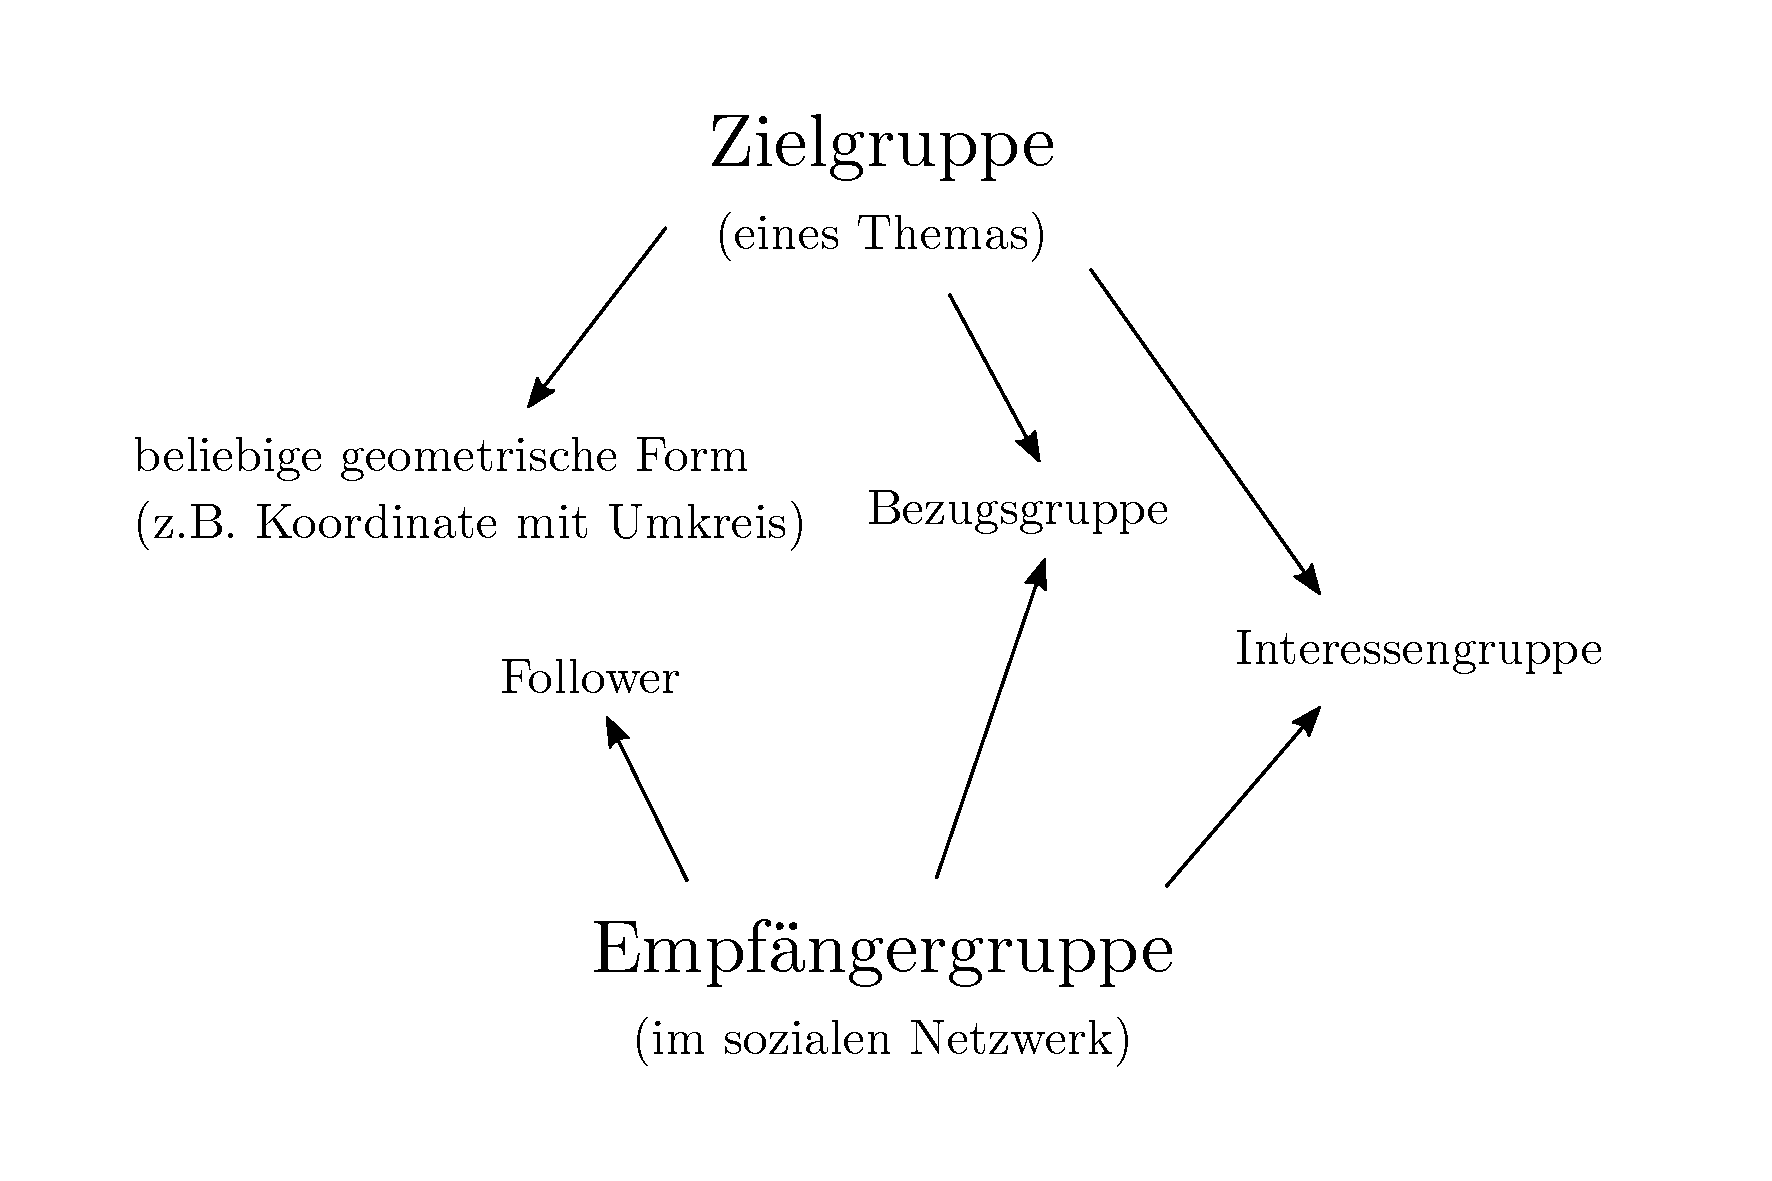
\includegraphics[width=0.8\textwidth]{zielgruppen_empfaengergruppen.pdf}
	\caption{Die Abbildung zeigt, welche Strukturen als Zielgruppen (in Bezug auf Themen) und welche als Empfängergruppen (in Bezug auf Posts im sozialen Netzwerk) existieren.}
	\label{fig.zielgruppen_empfaengergruppen}
\end{figure}

Jede reale Person kann ein Benutzerkonto erstellen, das aus einer frei wählbaren E-Mail-Adresse und einem Passwort besteht. Es gibt keine Möglichkeit Bilder, Benutzernamen oder andere persönliche Daten anzugeben.

Bei solchen anonymen Konten kann es durch Bot- und Troll-Benutzerkonten zu Missbrauch kommen. Auch kann der Entscheidungsprozess durch mehrere Benutzerkonten ein und derselben Person gezielt manipuliert werden. Ein \gls{benutzer} soll daher mit einem Karmawert $K$ bewertet werden, die es den anderen \glsdisp{benutzer}{Benutzern} erleichtern sollen, die Echtheit eines Benutzerkontos einzuschätzen. Der Karmawert setzt sich aus verschiedenen Teilwerten zusammen. Diese Teilwerte sind etwa Reputation (z.B. die Bilanz von Up- und Downvotes von Benutzerbeiträgen), Vertrauen (z.B. Größe und Isolation des sozialen Netzwerks) und/oder Positionsbestätigungen (z.B. Anzahl bestätigter Positionen, Anzahl bestätigter \glspl{bezugsgruppe}). Abhängig vom globalen Karmawert oder von Teilwerten bekommen die \glspl{benutzer} bestimmte Rechte erteilt oder entzogen (z.B. das Erstellen von \glspl{thema} oder das Downvoten von Kommentaren). Sinkt der globale Karmawert unter eine bestimmte Schwelle $K<K_\text{ban}$, so wird von einem unechten \gls{benutzer} ausgegangen und automatische Sperrmaßnahmen werden eingeleitet.

Um bereits vor der Anmeldung die Anzahl unechter Konten zu limitieren, werden \glspl{benutzer} nur über Einladungen zum Netzwerk zugelassen, wobei jedem \gls{benutzer} pro Zeiteinheit (z.B. pro Woche) nur eine bestimmte Anzahl an Einladungen (z.B. $1$) zur Verfügung steht.

\subsection{Soziales Netzwerk}

\glspl{benutzer} können sich untereinander vernetzen, um leichter interessante \glspl{thema} zu finden, inhaltliche Inspirationen zu sammeln und Neuigkeiten auszutauschen. Eine von einem \gls{benutzer} an sein soziales Umfeld abgesendete Information wird als \gls{post} bezeichnet. Ein \gls{post} kann auf eine \gls{bezugsgruppe} (siehe oben), eine \gls{interessengruppe} und/oder auf sogenannte \glspl{follower} als \gls{empf-gruppe} beschränkt werden (siehe Abb. \ref{fig.zielgruppen_empfaengergruppen}). \glspl{follower} und \glspl{interessengruppe} werden im Folgenden beschrieben.

\glspl{benutzer}, die an den \glspl{post} anderer \glspl{benutzer} interessiert sind, können diesen folgen; sie werden dann als \gls{follower} bezeichnet. Eine \gls{follower}-Beziehung ist unidirektional, d.h. sie erfolgt ohne gegenseitige Bestätigung und ist anonym. \glspl{benutzer} haben damit die Möglichkeit, auf einer Timeline von der Aktivität anderer \glspl{benutzer} zu erfahren. So erhalten sie Zugang zu potentiell \glsdisp{relevanz}{relevanten} \glspl{thema} und allgemeinen Informationen.

\glspl{benutzer}, die ein bestimmtes gemeinsames Interesse teilen, können sich in so genannten \glspl{interessengruppe} zusammenschließen, deren \glspl{mitglied} als \glspl{genosse} bezeichnet werden. Eine \gls{interessengruppe} wird von einem \gls{benutzer} gegründet und muss keinen eindeutigen Namen besitzen. Der gründende \gls{benutzer} ist automatisch Administrator der \gls{interessengruppe} und besitzt damit das Recht, anderen \glsdisp{benutzer}{Benutzern} Zugang zu gewähren. Ein Administrator kann weitere \glspl{benutzer} zu Administratoren ernennen, die \gls{interessengruppe} umbenennen und löschen. Ein \gls{thema} kann einer \gls{interessengruppe} als \gls{zielgruppe} zugeordnet werden, wodurch nur die \glspl{genosse} einer \gls{interessengruppe} \glspl{pot-teilnehmer} des \glsdisp{thema}{Themas} sind. Solche \glspl{thema} werden als geschlossene \glspl{thema} bezeichnet. Zusätzlich steht ein Forum zur Verfügung, um weiteren Austausch und Diskussionen zu ermöglichen. \glspl{genosse} einer \gls{interessengruppe} haben so zum Beispiel die Möglichkeit, sich gegenseitig auf potentiell \glsdisp{relevanz}{relevante} \glspl{thema} aufmerksam zu machen, gemeinsam neue \glspl{thema} vorzubereiten und ein geschlossenes Vorgehen bei \glspl{thema} zu koordinieren.

\newpage

%%%%%%%%%%%%%%%%%%%%
%%%%% APPENDIX %%%%%
%%%%%%%%%%%%%%%%%%%%

\section{Appendix}

\begin{table}[!h]
    \footnotesize
    \centering
    \begin{tabular}{p{.45\textwidth}p{.02\textwidth}p{.45\textwidth}}
      \textbf{Bezugsgruppe}   && \textbf{Interessengruppe} \\  [+0.5em] \hline
      
      Dezentral organisiert  & & Zentral organisiert \\ \hline
      
      Kann als Empfängergruppe für \glspl{post} im sozialen Netzwerk dienen & & Kann als Empfängergruppe für \glspl{post} im sozialen Netzwerk dienen \\ \hline
      
      Kann als \gls{zielgruppe} für \glspl{thema} dienen && Kann als \gls{zielgruppe} für \glspl{thema} dienen \\ \hline
      
      Kann einem \gls{thema} zugeordnet werden, das \gls{thema} wird als offen markiert && Kann einem \gls{thema} zugeordnet werden, das \gls{thema} wird als geschlossen markiert \\ \hline
      
      Offen, d.h. prinzipiell zugänglich für alle && Geschlossen, d.h. nur zugänglich für freigeschaltete Personen \\ \hline
      
      Unverwaltet; es gibt keinen Administrator, \gls{bezugsgruppe} kann ``entstehen und vergehen'' && Verwaltet; Administratoren entscheiden über Aufnahme neuer \glspl{genosse}, Ernennung von Administratoren und Löschung/Umbenennung der \gls{gruppe} \\ \hline
      
      Verifizierung dezentral durch andere \glspl{benutzer} über Algorithmus && Verifizierung zentral durch einen/mehrere Administrator/en \\ \hline
      
      Name ist eindeutig, ``\#hessen'' kann nur einmal existieren && Name ist nicht eindeutig, “Hessen” kann mehrfach vorkommen, nur ID ist eindeutig \\ \hline
      
    \end{tabular}
    \caption{Unterschiede zwischen Bezugs- und Interessengruppen}
    \label{tab:difference-bg-ig}
\end{table}

\newpage

%%%%%%%%%%%%%%%%%%%
%%%%% GLOSSAR %%%%%
%%%%%%%%%%%%%%%%%%%

\printglossaries

\end{document}
